\documentclass{acmsiggraph}               % final

%% These two line bring in essential packages: ``mathptmx'' for Type 1
%% typefaces, and ``graphicx'' for inclusion of EPS figures.


\usepackage{graphicx}
\usepackage{url}
\usepackage{times}
\usepackage{float}
\usepackage{amsmath}
\usepackage{mathtools}



%% Paper title.

\title{Temporal Reprojection Anti-Aliasing}

%% Author / Affiliation (single author).

%%\author{Roy G. Biv}
%%\affiliation{Allied Widgets Research\thanks{email:roy.g.biv@aol.com}}

%% Author / Affiliation (multiple authors).

\author{Christian Alexander Oliveros Labrador\thanks{e-mail: christianol\_01@hotmail.com} %%\and Second Author\thanks{second.author@cs.lth.se}
}
\affiliation{Lund University\\ Sweden}


%% Keywords that describe your work.
\keywords{Temporal Reprojection Anti Aliasing TAA TXAA TRAA}

%%%%%% START OF THE PAPER %%%%%%

\begin{document}

\ifpdf
  \DeclareGraphicsExtensions{.jpg,.pdf,.mps,.png}
\else
  \DeclareGraphicsExtensions{.eps}
\fi


\maketitle

\begin{abstract}
In this essay, I describe the implementation of Temporal Reprojection Anti-Aliasing (TRAA) I implemented for the EDAN35 High Performance Computer Graphics project. 
It is based on the Pedersen TRAA article for their game, Inside ~\cite{Fuglsand2016}, and on the Xu TAA article for their game, Uncharted 4 ~\cite{XU2016}.

\end{abstract}


\section{Introduction}
The Aliasing problem that computer graphics experience comes from not being able to sample as required by the Nyquist-Shannon Sampling Theorem, creating ragged edges that appear in the rasterization process (Spatial Aliasing) and jumps between moving objects (Temporal Aliasing), according with Doggett and Wronski  ~\cite{Doggett2017,Wronski2014}. Many solutions have been proposed and used to solve it, e. g. the Super Sampling Anti-Aliasing (SSAA) family of solutions that work on higher frequencies than the required at the cost of more space  requirements. 

The motivation of this project is to  implement a solution from the Temporal Reprojection Anti-Aliasing family, which is relatively new and promises to solve spatial and temporal aliasing problems in post processing ~\cite{Fuglsand2016} using less memory requirements than the SSAA family while keeping the same quality. This is done using the variation between the current frame and past ones to refine the output image.

\section{Algorithms}
Camera Jitter; Velocity Buffer; Frame History Buffer; Clipping Color Box; Sharpen Filter; and Motion Blur are used to implement the TRAA.
\subsection{Camera Jitter}
Camera Jitter is applied every frame to preserve information from local regions of surface fragments. If the current frame is static relative to the past ones then the system is loosing information that could use to refine it. ~\cite{Fuglsand2016,XU2016}
\begin{figure}[H]
    \centering
    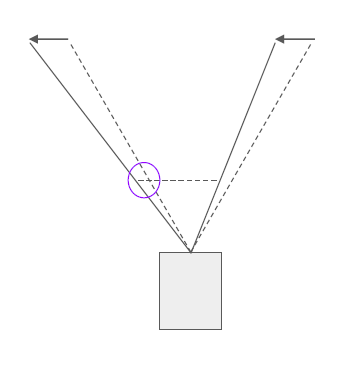
\includegraphics[scale=0.3]{Jitter.png}
    \caption{Jittering the Projection Matrix. Image taken from \protect\cite{Fuglsand2016}}
    \label{fig_Jitter}
\end{figure}

The jittering is applied as a translation to the projection matrix using the Halton Sequence (2,3) as the translation deltas. This sequence is used because it is better to have an irregular pattern for the translations ~\cite{Fuglsand2016,XU2016}. 
\begin{figure}[H]
    \centering
    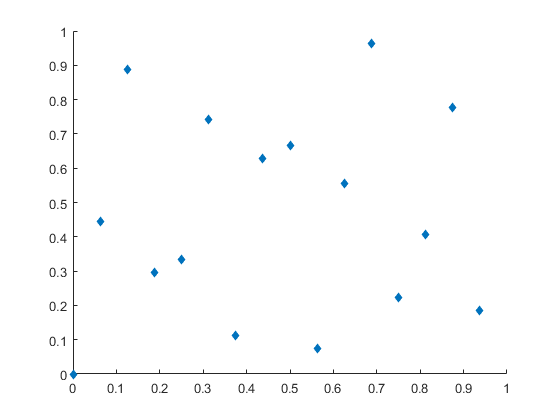
\includegraphics[scale=0.3]{Halton.png}
    \caption{Values from the Halton Sequence (2,3) used}
    \label{fig_Halton}
\end{figure}
The Figure~\ref{fig_Halton} is the representation of the 16 points used to jitter the projection in my implementation, as proposed by Pedersen ~\cite{Fuglsand2016}. It was generated using MATLAB with the command haltonset(2) then scrambled using reverse-radix scrambling, scramble(p, 'RR2') and, finally, generated the 16 points used with net(p, 16).

\subsection{Velocity Buffer}
The Velocity Buffer algorithm used in this implementation is the one proposed by Chapman ~\cite{Chapman2012} which is calculated by subtracting in NDC space the current pixel position by its last frame position. This is possible by saving the MVP matrix of each object in the scene.

Also, as suggested by Xu ~\cite{XU2016}, the jittering is not included as part of the motion.

\subsection{Frame History Buffer}
For each fragment in the current frame we look for the 3x3 neighborhood and plus (+) pattern neighborhood (See Figure~\ref{fig_Pattern}). On both patterns we look for the minimum and maximum of colors of the current frame, later we average them and use them in the Clipping of History ~\cite{Fuglsand2016}.

\begin{figure}[H]
    \centering
    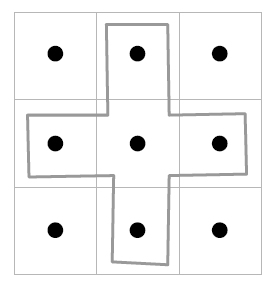
\includegraphics[scale=0.3]{Pattern.png}
    \caption{Sampling Pattern used. Image taken from \protect\cite{Fuglsand2016}}
    \label{fig_Pattern}
\end{figure}

On the 3x3 neighborhood we look for the velocity of the pixel with the closest depth, this is to get better edges in motion for pixels that are occluded ~\cite{Fuglsand2016}. We use this velocity to reproject the position of the current frame in the history ~\cite{Fuglsand2016,XU2016}.

After we have the history we constrain it (See next subsection) and we mix it with the current frame. We linearly mix both of them using a feedback value thats calculated by the difference of luminance between colors. This feedback is clamped between values closer to one to add some information of the current frame while keeping the history. This mix stabilizes the image, removing the jittering and smoothing the edges ~\cite{Fuglsand2016,XU2016}. Because history is accumulated, we get the effect that each frame weights less the more time the history is not rejected ~\cite{Fuglsand2016}.


\begin{figure}[H]
    \centering
    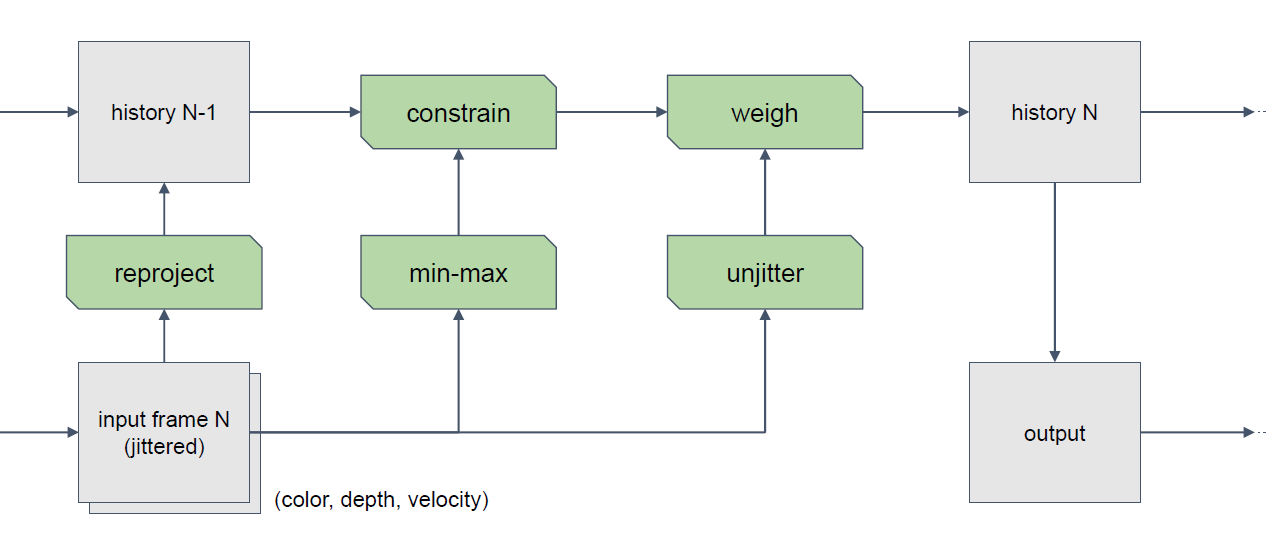
\includegraphics[width=0.9\columnwidth]{Process.png}
    \caption{Temporal Reprojection Anti-Aliasing process. Image taken from \protect\cite{Fuglsand2016}}
    \label{fig_Process}
\end{figure}

\subsection{Clipping Color Box}
To handle color rejection when history is too distant from current color a Clipping Color Box is used. This is a box built using the current pixel color as the center and the minimum and maximum color calculated in the last subsection as limits. The history color is taken as a position and projected against the limits of the box if it lies outside, else, it is left untouched. The use of the Clipping Color Box is to prevent color clustering that would happen if Clamp is applied (See Figure~\ref{fig_Constraint})~\cite{Fuglsand2016}.

\begin{figure}[H]
    \centering
    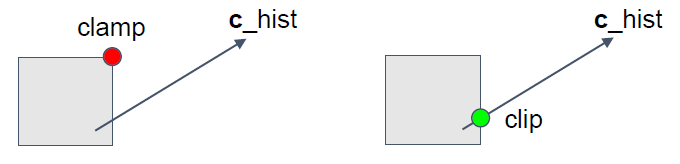
\includegraphics[width=0.9\columnwidth]{Constraint.png}
    \caption{Color Clamping versus Color Clipping. Image taken from \protect\cite{Fuglsand2016}}
    \label{fig_Constraint}
\end{figure}

\subsection{Sharpen Filter}
Because the Reprojection process and Color Clipping create blurriness, a Sharpen Filter is required. I used the one proposed by Xu ~\cite{XU2016}.
\begin{figure}[H]
	\centering
    \[
    \begin{bmatrix*}[r]
      0 & -1 &  0 \\
      -1 &  5 & -1 \\
      0 & -1 &  0
    \end{bmatrix*}
    \]
    \caption{Sharpen Filter Convolution Matrix. As used in \protect\cite{XU2016}}
	\label{fig_Sharpen}
\end{figure}

\subsection{Motion Blur}
Because the nature of the History Buffer, ghosting is created by fragments from objects that move so fast that they are not rejected as quickly as necessary under special lighting and background conditions. The proposed solution by Pedersen and Xu ~\cite{Fuglsand2016,XU2016} is to use Motion Blur to hide this artifacts.

The Motion Blur used is the one proposed by Chapman ~\cite{Chapman2012}. It tries to behave like a real camera by scaling the velocity of each pixel by the division of the current FPS to the one wanted, thus, simulating the shutter speed. Then it mixes the colors of the pixels that are sampled while following the direction of the velocity buffer vector.

\section{Results}
Results are shown in the next figures. All of them are renders of the Sponza scene.

\begin{figure}[H]
    \centering
    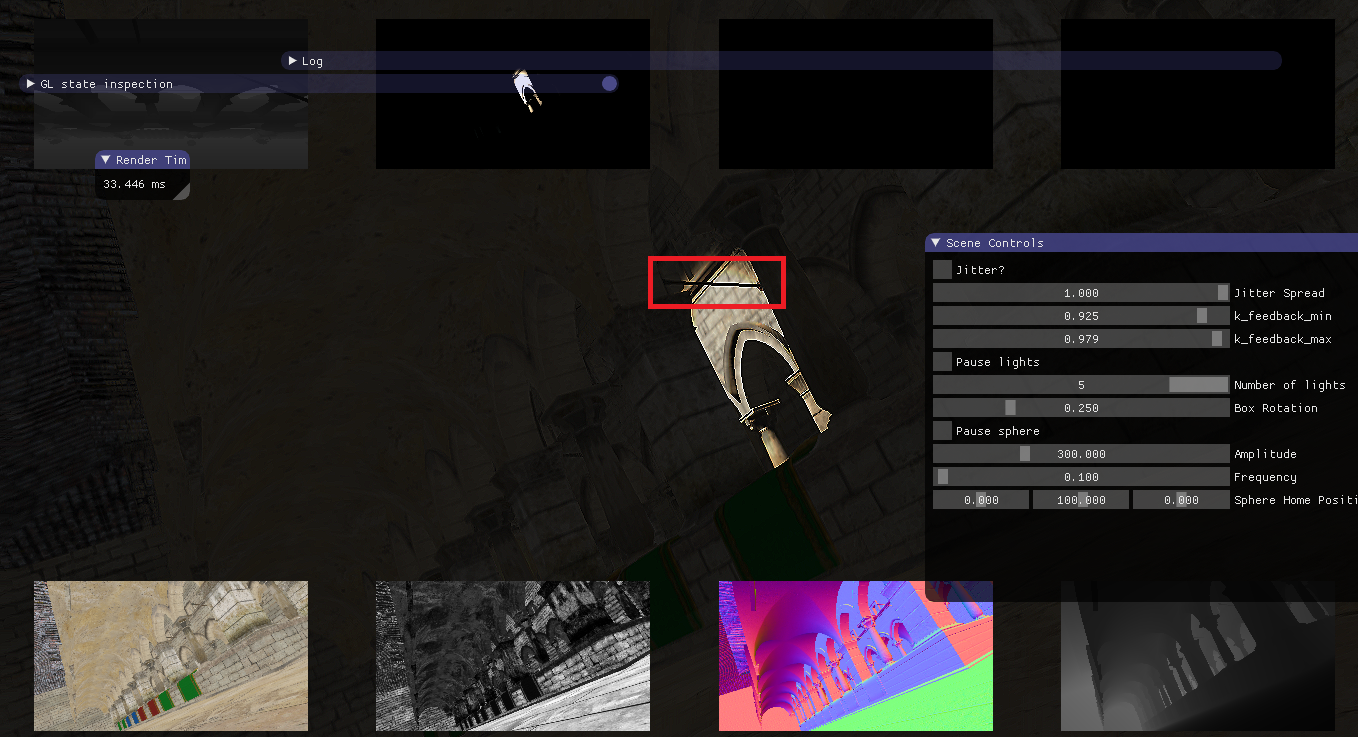
\includegraphics[width=0.9\columnwidth]{NO_AA.png}
    \caption{Bar Rendered without Anti-Aliasing}
    \label{fig_NO_AA}
\end{figure}

\begin{figure}[H]
    \centering
    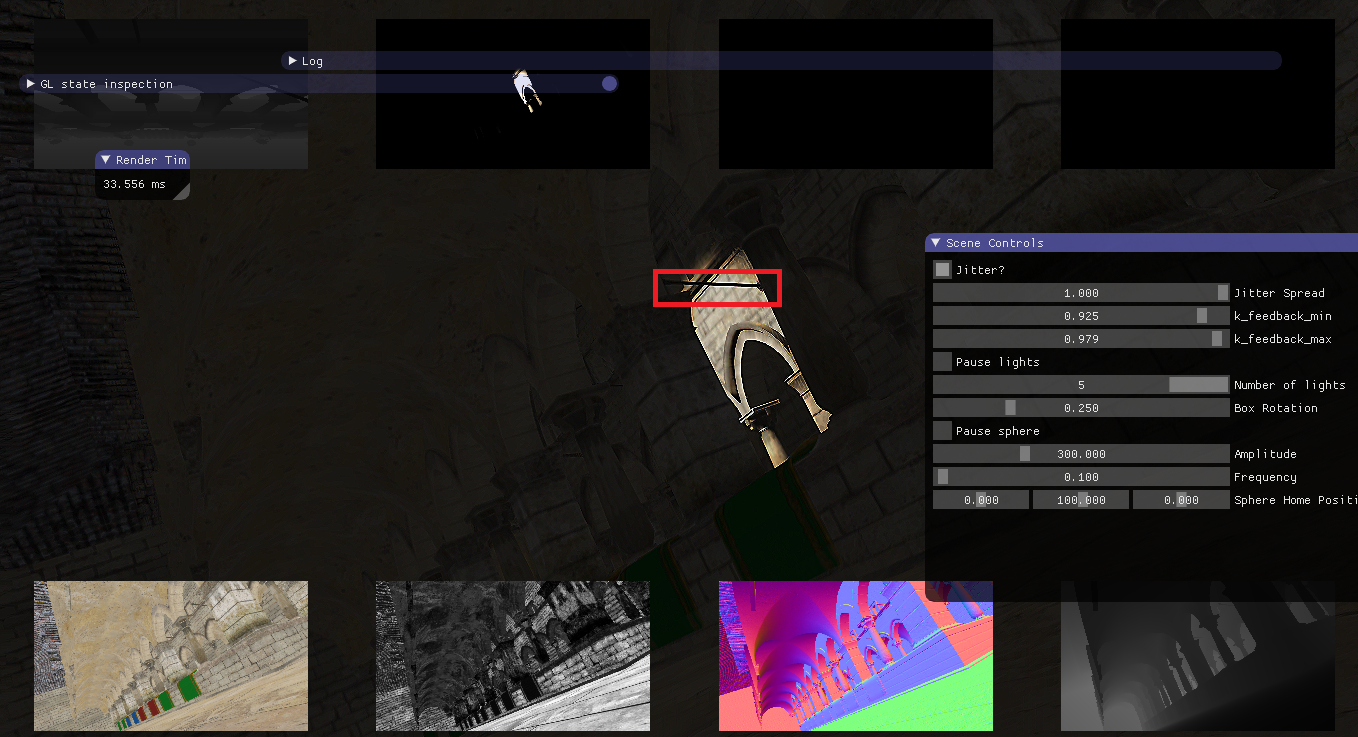
\includegraphics[width=0.9\columnwidth]{TRAA.png}
    \caption{Bar Rendered with TRAA}
    \label{fig_TRAA}
\end{figure}

\begin{figure}[H]
    \centering
    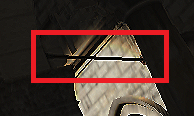
\includegraphics[width=0.9\columnwidth]{NO_AA_Zoom.png}
    \caption{Bar Rendered without Anti-Aliasing Zoomed}
    \label{fig_NO_AA_Zoom}
\end{figure}

\begin{figure}[H]
    \centering
    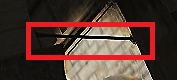
\includegraphics[width=0.9\columnwidth]{TRAA_Zoom.png}
    \caption{Bar Rendered with TRAA Zoomed}
    \label{fig_TRAA_Zoom}
\end{figure}

\begin{figure}[H]
    \centering
    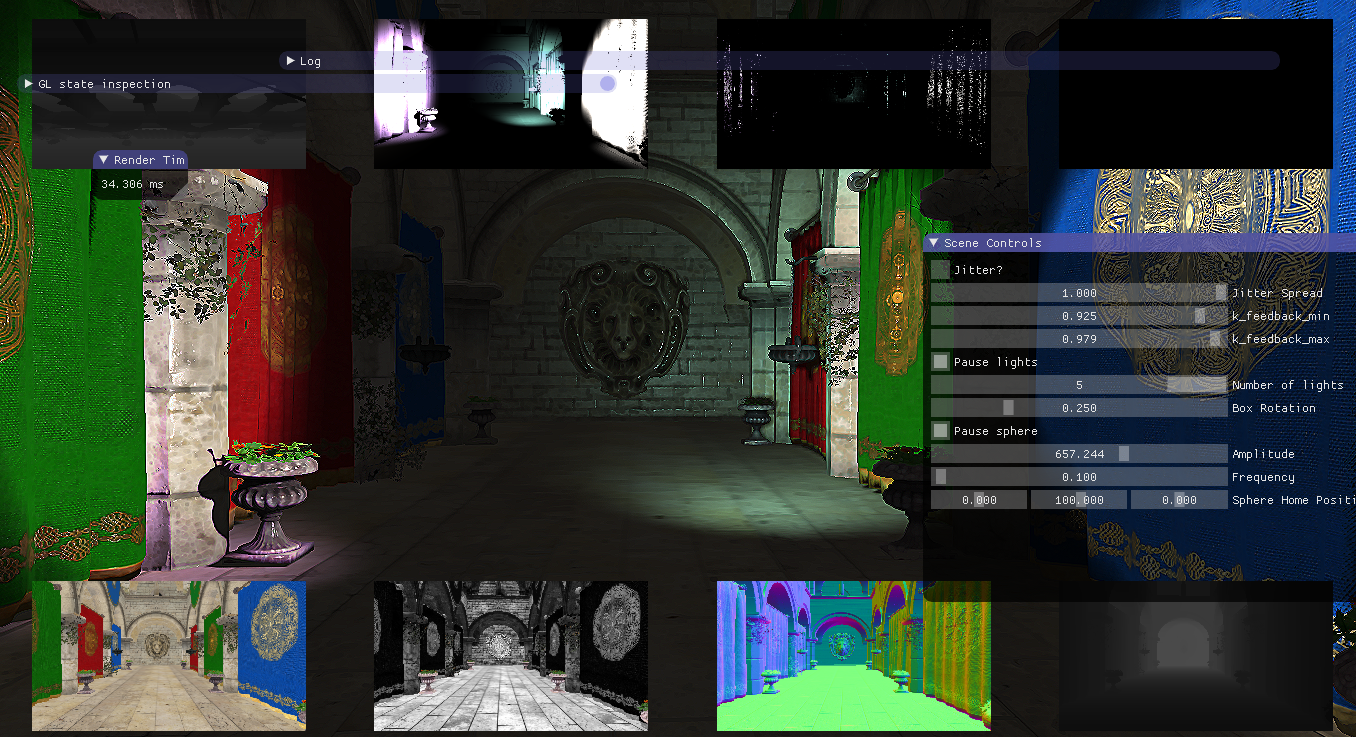
\includegraphics[width=0.9\columnwidth]{NO_AA_2.png}
    \caption{Sponza Render without Anti-Aliasing}
    \label{fig_NO_AA_2}
\end{figure}

\begin{figure}[H]
    \centering
    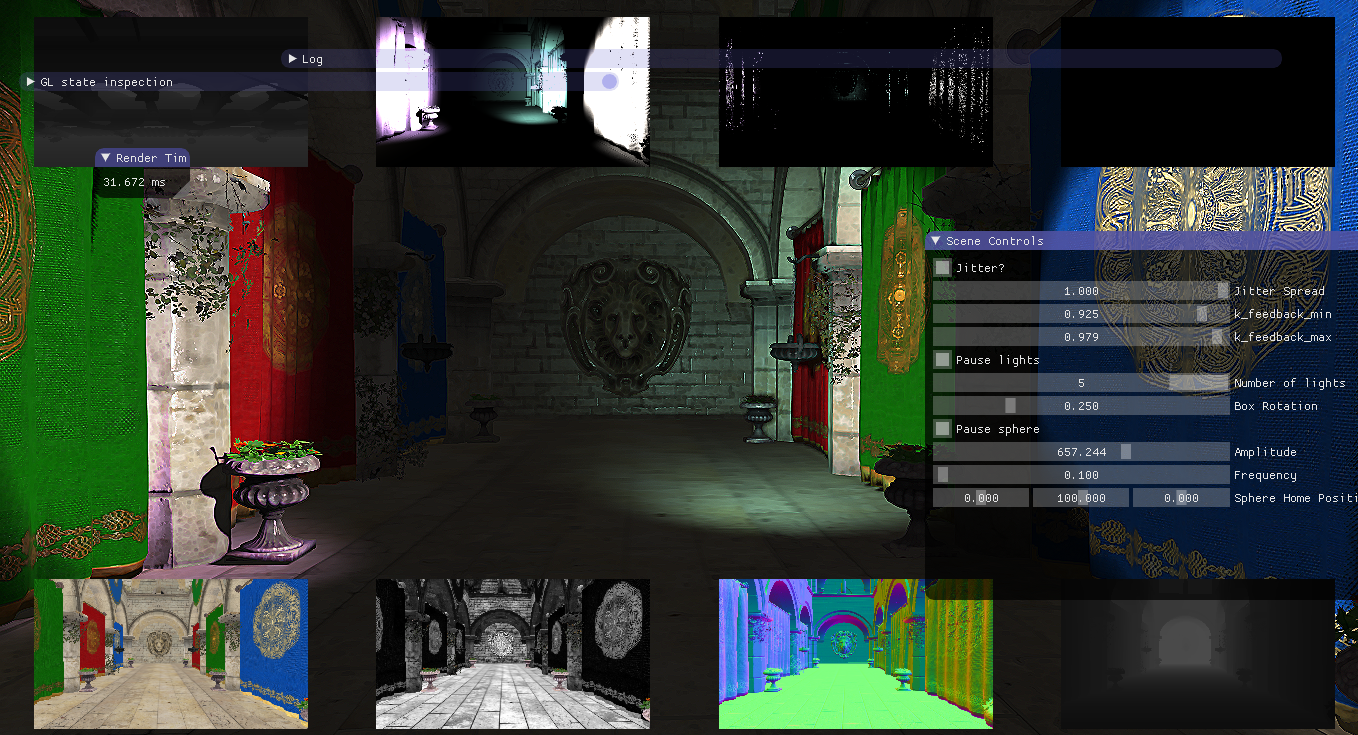
\includegraphics[width=0.9\columnwidth]{TRAA_2.png}
    \caption{Sponza Render with TRAA}
    \label{fig_TRAA_2}
\end{figure}

As we can see, the TRAA smoothes the edges of the images without a loss of quality or performance. 

\section{Discussion}
Current advances in TRAA allows its use in real time computer graphics without a great loss of performance while achieving good quality rendering. But it contain artifacts that affect the quality of the render.

\subsection{Blurriness}
The current implementation of TRAA generates a very aggressive  blur, needing a Sharpen Filter. 

I tried the Sobel Filter to control the blend of the current frame and the history based on where the edges where, but it created too many jittering artifacts. Also, I tried with a 5x5 Sharpen Filter but it changed the brightness too much.

The Sharpen Filter that was finally used in the implementation is the one used by Xu ~\cite{XU2016}, it solves the blurriness really well but it can not eliminate some artifacts. For future implementations I propose to try other Sharpen Filters, maybe one with a bigger kernel. Also, it might be possible to use the Sobel Filter to contrast edges.

\subsection{Jittering}
The current implementation of TRAA is fast to stabilize the image and cancel the jittering. But, it still has problems handling Specular Reflections that are close to the size of just one pixel. I propose to solve jittering by blurring a little the Specular Texture in the Deferred Resolve Pass to avoid pixel size Specular Reflections.

\subsection{Ghosting}
Some Ghosting is created when animation is done in particular special lighting and background conditions. This is partially corrected with motion blur but requires more processing to completely solve it completely. Xu proposes the use of Motion Blur and increase the size of everything by the use of an Stencil technique ~\cite{XU2016}. This is not used for the current implementation. 

Pederson implementation allows the jitter in the Velocity Buffer calculations but it creates some unwanted blurriness ~\cite{Fuglsand2016}. This could be another possible solution if the Sharpen Filter can remove that blurriness afterwards.

\section{Conclusion}
In conclusion Temporal Reprojection Anti-Aliasing is a good technique to solve the Aliasing problem in real time without incurring in heavy space or time requirements. Further research is needed to improve the image quality and reduce the ghosting, jittering and blurriness artifacts. 

\bibliographystyle{acmsiggraph}
%\nocite{*}
\bibliography{project}
\end{document}
